\documentclass{article}

\usepackage[reqno]{amsmath} % Paquete para el manejo de expresiones matemáticas [reqno], [leqno] y [fleqn]
\usepackage{amsthm}
\usepackage{amssymb,amsmath,latexsym} %Paquete para llamar símbolos matemáticos
\usepackage{amsfonts}
\usepackage[mathscr]{euscript}
\usepackage{graphicx} %paquete para el manejo de transformaciones geométricas de imagénes
\usepackage{color} %paquete para el manejo de color en textos.
%\usepackage[utf8]{inputenc} %paquete para el manejo de caracteres acentuados
\usepackage[french,spanish]{babel} %paquete que genera documentos en diferentes idiomas
\usepackage{enumerate}
\usepackage{multicol} % Paquete para modificar el número de columnas
\usepackage{layout} % Paquete  para revisar los valores de 
\usepackage{verbatim}
\usepackage[all]{xy} 
\usepackage{pgfplots}
%graficos
\usepackage{pgfplots}
\pgfplotsset{compat=1.15}
\usepackage{mathrsfs}
\usetikzlibrary{arrows}
\pagestyle{empty}
%graficos
\pagestyle{myheadings}  % Estilo de página
%\pagenumbering{arabic} % Estilo de numéración
\hoffset1cm
\newcounter{Teorema}
\newcommand{\Teorema}{\stepcounter{Teorema}{\bf Teorema \theTeorema.} }
\DeclareMathOperator{\arcsec}{arcsec} % Creación de nuevos comandos en latex
\DeclareMathOperator{\Var}{Var}
\DeclareMathOperator*{\Hom}{Hom}
\setcounter{MaxMatrixCols}{15}
\allowdisplaybreaks % Control de cambios de página en alineaciones
\decimalpoint
%\renewcommand{\theequation}{\thesection.\arabic{equation}}
\numberwithin{equation}{section}
%\renewcommand{\theequation}{\theparentequation\arabic{equation}}
%% Nuevos teoremas
\theoremstyle{plain}  % Requiere el paquete amsthm
\newtheorem{thm}{Teorema}[section]
\newtheorem{Corol}[thm]{Colorario}
\newtheorem{Prop}[thm]{Proposición}
\newtheorem{axiom[thm]}{Axioma}
\newtheorem{conj}{Conjetura}
\newtheorem{Def}{Definición}[section]
\newtheorem{Ej}{Ejemplo}[section]
\newtheorem{notacion}[Def]{Notación}
\newtheorem{nota}[Def]{Nota}
\renewcommand{\qedsymbol}{$\heartsuit$}
\providecommand{\abs}[1]{\lvert#1\rvert} %valor absoluto
\providecommand{\norm}[1]{\lVert#1\rVert} %norma
\usepackage{fancyhdr}
\pagestyle{empty}
\usepackage{pgfplots}
\usepackage{mathrsfs}
\usepackage{tcolorbox}
\usepackage{amsmath, amsthm, amssymb}
\usepackage{mathrsfs}
\usepackage{graphicx}
\usepackage{geometry}
\usepackage{multicol}
\usepackage{amsmath}
\spanishdecimal{.}
\usepackage{color}
\usepackage{multicol}
\usepackage{bbding}
\usepackage{stackrel}
\usepackage{hyperref}
\usepackage{geometry}
\usepackage{multicol}
\usepackage{amsmath}
\usepackage{amsfonts}
\usepackage{amssymb}
\usepackage{multicol}
\usepackage{bbding}
%\usepackage[manejador]{color,graphicx}

%colores 
\definecolor{dorado}{cmyk}{0,0.10,0.84,0}
\definecolor{melon}{cmyk}{0,0.29,0.84,0}
\definecolor{naranja}{cmyk}{0,0.42,1,0}
\definecolor{durazno}{cmyk}{0,0.46,0.50,0}
\definecolor{fresa}{cmyk}{0,1,0.50,0}
\definecolor{ladrillo}{cmyk}{0,0.77,0.87,0}
\definecolor{violeta}{cmyk}{0.07,0.90,0,0.34}
\definecolor{purpura}{cmyk}{0.45,0.86,0,0}
\definecolor{aguamarina}{cmyk}{0.85,0,0.33,0}
\definecolor{esmeralda}{cmyk}{0.91,0,0.88,0.12}
\definecolor{pino}{cmyk}{0.92,0,0.59,0.25}
\definecolor{oliva}{cmyk}{0.64,0,0.95,0.40}
\definecolor{canela}{cmyk}{0.14,0.42,0.56,0}
\definecolor{cafe}{cmyk}{0,0.81,1,0.60}
\definecolor{marron}{cmyk}{0,0.72,1,0.45}
\definecolor{gris-claro}{cmyk}{0,0,0,0.30}
\definecolor{gris-oscuro}{cmyk}{0,0,0,0.50}


\begin{document}
\pagestyle{empty}
%\afterpage{\blankpage}
\begin{center}
\begin{figure}[h]
\centering


\end{figure}
\Large
\hrule
\vspace{4mm}
\begin{center}
    
\includegraphics[scale=0.1]{ud.png}
\end{center}
\textbf{Ejercicio Final Introducción Al \LaTeX}\\

\vspace{4mm}
\hrule
\large
\vfill
Autor\\

Wilson Eduardo Jerez Hernández \\
20181167034\\ 
wejerezh@correo.udistrital.edu.co\\
\vfill
Profesor\\
Jhonatan Steven Mora Rodriguez.

\vfill
Universidad Distrital Francisco José de Caldas
\\
Facultad de Ciencias y Educación\\
Matemáticas \\
\end{center}
\newpage


\addtocontents{toc}{\hfill \textbf{Página} \par}
\tableofcontents
\newpage

	
\pagestyle{fancy}
\pagenumbering{gobble}
\rfoot{Universidad Distrital José Francisco de Caldas\\
		Facultad Ciencias y Educación\\
		Proyecto de Matemáticas}
\mbox{}	
\lhead[]{}
\newpage
%%%%%%%%%%%%%%%%%%%%%%%%%%%%%%%%%%%%%%%%%%%%%%%%%%%%%%%%%%%%%
\section{La Ecuación de Clase}
Antes de hablar de la Ecuacion de clase vamos a demostar el siguiente teorema. 
\begin{thm}
Sea $G$ un grupo finito y sea $X$ un G-conjunto finito. si $x  \in X$, entonces $\abs{O_{x}} = [G : G_{x}]$.

\vspace{5mm}
\textbf{Demostración.}
\vspace{5mm}

Sabemos que $\abs{G}/\abs{G_{x}} $
es el número de clases laterales iz1quierdas de $G_{x}$ en $G$ por el Teorema de Lagrange .
Definemos una función biyectiva $\phi$ de la órbita $O_{x}$ de x al conjunto de clases laterales izquierdas $L_{G_{x}}$ de $G_{x}$ en $G$. Sea $y \in O_{x}$. ENtonces existye $g$ en $G$ tal que $gx=y$. Definamos $\phi$ de forma que $\phi(y) = gG_{x}.$ Para mostrar que $\phi$ es $1-1$, supongamos que $\phi(y_{1}) = \phi(y_{2})$. Entonces
\begin{equation*}
    \phi(y_{1}) = g_{1}G_{x} = g_{2}G_{x} = \phi(y_{2}),
\end{equation*}
donde $g_{1}x = y_{1}$ y $g_{2}x = y_{2}$. Como $g_{1}G_{x} = g_{2}G_{x}$, existe $g \in G_{x}$ tal que $g_{2} = g_{1}g$,
\begin{equation*}
    y_{2} = g_{2}x = g_{1}gx = g_{1}x = y_{1};
\end{equation*}
por lo tanto. la función $\phi$ es 1-1. Finalmente, debemos mostrar que $\phi$ es epiyectiva. sea $gG_{x}$ una clase lateral izquierda. Si $gx=y$, entonces $\phi(y) = gG_{x}.$ \textbf{QED}
\end{thm}
%%%%%%%%%%%%%%%%%%%%%%%%%%%%%%%%%%%%%%%%%%%%%%%%%%%%%%%%%
Sea $X$ un G- conjunto y $X_{G}$ el conjunto de puntos fijos en $X$; es decir, 
\begin{equation*}
    X_{G} = \{x \in X : gx = x \text{ para todo }  g \in G\}. 
\end{equation*}
Como las órbitas de la acción particionan a $X$, 
\begin{equation*}
    \abs{X} = \abs{X_{G}}+ \sum_{i =k}^{n}\abs{O_{x_{i}}}
\end{equation*}
donde $x_{k},\cdots,x_{n}$ son representantes de las distintas órbitas no triviales de 
$X$ (aquellas órbitas que contienen más de un elemento). \vspace{5mm}

Ahora consideremos el caso especial en el que G actua en sí mismo por conjugación, $(g,x) \to gxg^{-1}$. El \textbf{centro} de $G$, 
\begin{equation*}
    Z(G) = \{ x : xg = gx \text{ para todo } g \in G\},
\end{equation*}

es el conjunto de puntos que quedan fijos por conjugación. La órbitas de la acción se llaman \textbf{clases de conjugación} de $G$. Si $x_{1},\cdots,x_{k}$ on representantes de cada una de las clases de conjugación no-triviales de $G$ y $\abs{O_{x_{1}}}= n_{1}, \cdots , \abs{O_{x_{k}}} = n_{k}$, entonces
\begin{equation*}
    \abs{G} = \abs{Z(G)} + n_{1} + \cdots + n_{k}.
\end{equation*}
Cada uno de los subgrupos estabilizadores de uno de los $x_{i}$, $C(x_{i}) = \{g \in G : gx_{i} = x_{i}g\}$, se llama \textbf{subgrupo centralizador} de $x_{i}$. Por el \textbf{Teorema 1.1}, obtemos la \textbf{ecuación de clase:} 
\begin{equation*}
    \abs{G} = \abs{Z(G)} + [G:C(x_{1})] + \cdots + [G:C(x_{k}].
\end{equation*}
Una de las conseciuencias de la ecuación de clase es que el orden de cada clase de conjugación divide al orden de $G$.
%%%%%%%%%%%%%%%%%%%%%%%%%%%%%%%%%%%%%%%%%%%%%%%%%%%%%%%%%
\section{Los teoremas de Sylow}
Recordemos Por un momento lo que significa que $G$ actúe en si mismo por conjugación y cómo las clases de conjugación se distribuyen en el grupo de acuerdo  a la ecuación de clase, discutida anterioremnte. 
Un grupo $G$ actúa en si mismo por conjugación de manera que $(g,x) \to gxg^{-1}$. 
Sean $x_{1}, \cdots , x_{k}$ representantes de cada una de las distintas clases de conjugación de $G$ que contiene más de un elemnto. Entonces la ecuación de clase se escribe como
\begin{equation*}
    \abs{G} = \abs{z(G)} + [G:C(x_{1})] + \cdots + [G: C(x_{k})], 
\end{equation*}
donde $Z(G) = \{g \in G : gx = xg \text{ para todo } x \in G\}$ es el centro de $G$ y $C(x_{i}) = \{ g \in G : gx_{i} = x_{i}g\}$ es el subgrupo centralizador de $x_{i}$. 
\vspace{5mm}low examinando los subgrupos de orden $p$, donde $p$ es un primo. Un grupo de $G$ es un \textbf{P-grupo} si todo elemneto de $G$ tiene orden potencia de $p$, donde $p$ es un  número primo. Un subgrupo de un grupo $G$ es un \textbf{P-subgrupo} si es un p-grupo. 
\begin{thm}
(cauchy) sea $G$ un grupo finito y P un primo tal que p divide el orden de $G$. Entonces $G$ contiene un elemnto de orden p.

\vspace{5mm}
\textbf{Demostración}
\vspace{5mm}

Procederemos por inducción sobre el orden de $G$. si $\abs{G}=p$, entonces un generados de $G$ es el elemnto requerido. Supongamos ahora que todo subgrupo de orden $k$, donde $p \leq k < n$ y $p$ divide a $k$, tiene un elemnto de orden $p$. supongamos que $\abs{G} = n$ y que $p | n$ y consideremos la ecuación de clase de $G$: 
\begin{equation*}
    \abs{G} = \abs{z(G)} + [G:C(x_{1})] + \cdots + [G: C(x_{k})]
\end{equation*}
Tenemos dos casos que considerar. 

\vspace{5mm}
\textbf{Caso 1.} el orden de alguno de los subgrupos centralizadores, $C(x_{i})$, es divisible por $p$ para algún $i, i = 1, \cdots, k.$ En este caso, por hipótesis de inducción estamos listos. Como $C(x_{i})$ es un subgrupo propio de $G$ y $p$ divide a $\abs{C(x_{i})}$, $C(x_{i})$ contiene un elemnto de orden $p$. Por lo tanto, $G$ contiene un elemnto de orden $p$. 

\vspace{5mm}
\textbf{Caso 2.} Ninguno de los centralizadores tiene orden divisible por $p$. Entonces $p$ divide a $[G:C(x_{i})]$, el orden de cada clase de conjugación en la ecuación de clase; luego, $p$ divide el orden del centro de $G$, $Z(G)$. Como $Z(G)$ es abeliano, tiene un subgrupo de orden $p$ por el Teorema Fundamental de Los Grupos Abelianos Finitos. Por lo tanto, el centro de $G$ contiene un elemnto de orde $p$.
\end{thm}
\begin{Corol}
Sea $G$ un grupo finito. Entonces $G$ es un P-grupo si y solo si $\abs{G} = p^{n}.$
\end{Corol}
\begin{Ej}
Consideremos el grupo $A_{5}$. Sabemos que $\abs{A_{5}}= 60 = 2^{2}\cdot 3 \cdot 5$. por el Teorema de Cauchy, sabemos que $A_{5}$ tiene subgrupos de órdenes 2,3 y 5. Los teoremas de sylow nos daán aún más información sobre los posibles subgrupos de $A_{5}$
\end{Ej}
\vspace{5mm}
Podemos ahora enunciar el primer Teorma de Sylow. La demostración es muy similar a la del Teorema de Cauchy. 
\vspace{5mm}

\begin{thm}
(primer teorema de Sylow) Sea G un grupo finito y p un primo tal que $p^{r}$ divide a $\abs{G}$. Entonces G contiene un subgrupo de orden $p^{r}$
\vspace{5mm}
\textbf{Demostración} 
\vspace{5mm} Procederemos por inducción sobre el orden de   $G $  una vez más.
Si $\abs{G}=p$ ,entonces estamos listos. Ahora supongamos que el orden de $G$ es $n$ con 
$n > p$ y que el teorema es verdadero para todos los grupos de orden menor a $n$, donde $p$
divide a $n$.Usaremos la ecuación de clase una vez más: 
\begin{equation*}
    \abs{G}= \abs{Z(G)} + [G:C(x_{1})] + \cdots + [G:C(x_{k})].
\end{equation*}
Supongamos primero que $p$ no divide a $[G:C(x_{i})]$ para algún $i$.Entonces
$p^{r}\text{ | }\norm{C(x _{i})}$ , pues $p^{r}$ divide a 
$\abs{G} = \abs{C(x_{i})}\cdot [G:C(x_{i})]$. Podemos aplicar la hipótesis de inducción a $C(x_{i})$

\vspace{5mm}

Por lo tanto, podemos suponer que p divide a $[G:C(x_{i})]$ para todos los $i$.
Como p divide a $\abs{G}$, la ecuación de clase dice que p divide a $\abs{\abs{Z(G)}}$; 
luego, por el teorema de Cauchy,$Z(G)$ tiene un elemento de orden p,digamos g.
Sea N el grupo generado por g. Claramente, $N$ es un subgrupo normal de $Z(G)$   
pues  $Z(G)$ es abeliano; por lo tanto,N es normal en G pues todo elemento en $Z(G)$ 
conmuta con todo elemento en $G$. Ahora consideremos el grupo cociente $G/N$ de orden 
$\abs{G}/p$.Por la hipótesis de indicción, $G / N$ contiene un subgrupo $H $ de orden
$p^{r-1} $.La preimagen de $H$ bajo el homomorfismo canónico $\phi :G → G / N$ es un 
subgrupo de orden $p^{r}$ en $G$.
\end{thm}



\section{Sea $S_{n}$ el grupo simétrico de n-letras. \\ Demuestre que $A_{n} \trianglelefteq S_{n}$}
\textbf{Preliminares}\\
\begin{thm}
    Sea G un grupo y N un subgrupo de G. Son equivalentes las siguientes afirmaciones:
    \begin{enumerate}
        \item aN = N a para cada a $\in$ G.
        \item  Para cada a, b $\in$ G se tiene ab $\in$ N implica ba $\in$ N.
        \item $aNa^{-1}$ = \{$ana^{-1} $ tal que n $\in$ N\} $\subseteq$ N para cada a $\in$ G.
        \item $aNa^{-1}$ = N para cada a $\in$ G.
    \end{enumerate} 
\end{thm}
\begin{thm}


\begin{enumerate}
    \item una permutación par $\circ $ una permutación par es una una permutación par
    \item una permutación par $\circ $  una permutación impar es una permutaciónimpar
    \item una permutación impar $\circ $ una permutación par es una permutación impar
    \item una permutación impar $\circ $ una permutación impar es una permutación par
    
\end{enumerate}


\textbf{Demostración}\\
Sabemos que los $\sigma$ son pares o bien impares\\
\newline
\textit{caso 1} \\ sea $\sigma$ una permutación par entonces $\sigma =( (a_{1}a_{n})(a_{1}a_{n-1} ...(a_{1}a_{3})(a_{1}a_{2}) )$ consideremos pues a $\sigma^{-1} = ((a_{1}a_{2})^{-1}(a_{1}a_{3})^{-1}...(a_{1}a_{n-1})^{-1}(a_{1}a_{n})^{-1}$ puesto que $(ab)^{-1}= b^{-1}a^{-1}$ pero tambien sabemos que cualquier transposición es el inverso de si misma por lo tanto $\sigma^{-1} = ((a_{1}a_{2})(a_{1}a_{3})...(a_{1}a_{n-1})(a_{1}a_{n})$ y como el número de transposiciones de $\sigma^{-1}$ nunca cambia entonces $\sigma^{-1}$ es par y sea cualesquiera $\tau \in A_{n}$ por tanto $\tau$ es par y por lema 2 $\sigma \circ \tau$ es par y $\sigma \circ \tau \circ \sigma^{-1}$ es par por tanto $\sigma \circ \tau \circ \sigma^{-1}\subseteq A_{n}$ y por lema 1 $\sigma A_{n} = A_{n} \sigma$ para $\sigma$ par\\
\newline
\textbf{caso 2} \\
sea $\sigma$ una permutación impar entonces $\sigma =( (a_{1}a_{n})(a_{1}a_{n-1} ...(a_{1}a_{3})(a_{1}a_{2}) )$ consideremos pues a $\sigma^{-1} = ((a_{1}a_{2})^{-1}(a_{1}a_{3})^{-1}...(a_{1}a_{n-1})^{-1}(a_{1}a_{n})^{-1}$ puesto que $(ab)^{-1}= b^{-1}a^{-1}$ pero tambien sabemos que cualquier transposición es el inverso de si misma por lo tanto $\sigma^{-1} = ((a_{1}a_{2})(a_{1}a_{3})...(a_{1}a_{n-1})(a_{1}a_{n})$ y como el número de transposiciones de $\sigma^{-1}$ nunca cambia entonces $\sigma^{-1}$ es impar y sea cualesquiera $\tau \in A_{n}$ por tanto $\tau$ es par y por lema 2 $\sigma \circ \tau$ es impar y $\sigma \circ \tau \circ \sigma^{-1}$ es par por tanto $\sigma \circ \tau \circ \sigma^{-1}\subseteq A_{n}$ y por lema 1 $\sigma A_{n} = A_{n} \sigma$ para $\sigma$ impar\\
\newline
por \textbf{caso 1} y \textbf{caso 2} $\sigma A_{n} = A_{n} \sigma$ para cada $\sigma \in S_{n}$ $\hfill\square$.
\end{thm}
\section{Operaciones básicas con matrices}

    \subsection{Suma de matrices}
    Dadas dos matrices de la misma dimensión, $A=(a_{ij})$ y $B=(b_{ij})$, se difinen la matriz suma como:
    $A+B=(a_{ij}+b_{ij})$. Es decir aquella matriz cuyos elementos se obtienen umando los elementos de las 
    dos matrices que ocupan la misma misma posición, es decir,
    \begin{equation*}
        \begin{pmatrix}
            a_{1} & a_{2}\\
            a_{3} & a_{4}
        \end{pmatrix}
        + 
        \begin{pmatrix}
            b_{1} & b_{2} \\ 
            b_{3} & b_{4}
        \end{pmatrix}
        = 
        \begin{pmatrix}
            a_{1}+b_{1} & a_{2}+b_{2} \\ 
            a_{3}+b_{3} & a_{4}+b_{4}
        \end{pmatrix}
    \end{equation*}
    \subsection{Producto de un número real por una matriz} 
    Dada una matriz $A=(a_{ij})$ y un número real $\lambda$, 
    se define el producto de un número real por una matriz: a la matriz del mismo orden que 
    $A$, en la que cada elemento está multiplicado por $\lambda$.
    \begin{equation*}
        \lambda \cdot
        \begin{pmatrix}
            a_{1} & a_{2} \\ 
            a_{3} & a_{4}
        \end{pmatrix}
        =
        \begin{pmatrix}
            \lambda \cdot a_{1} & \lambda \cdot a_{2} \\ 
            \lambda \cdot a_{3} & \lambda \cdot a_{4}
        \end{pmatrix}
    \end{equation*}
    \subsection{Producto de matrices}
    Dos matrices $A$ y $B$ se dicen multiplicables si el número de columnas de $A$ coincide con el número de filas de $B$.
    \begin{equation*}
        A_{m\times n} \times B_{n\times p} = M_{m\times p}
    \end{equation*}

    El elemento $c_{ij}$ de la matriz producto se obtiene multiplicando cada elemento de la fila $i$ de la matriz 
    $A$ por cada elemento de la columna $j$ de la matriz $B$ y sumándolos.
\section{tabla de distribución normal}
Para poder utilizar la tabla tenemos que transformar la variable $X$ que sigue una distribución $N(\mu, \sigma)$ 
en otra variable $Z$ que siga una distribución $N(0, 1)$\\
\begin{tabular}{|c|c|c|c|c|c|c|c|c|c|c|} 
\hline
z	& 0.00	&0.01	&0.02	&0.03	&0.04	&0.05	&0.06	&0.07	&0.08	&0.09   \\ \hline
0.0	& 0.5000&0.5040	&0.5080	&0.5120	&0.5160	&0.5199	&0.5239	&0.5279	&0.5319	&0.5359\\
0.1	& 0.5398&0.5438	&0.5478	&0.5517	&0.5557	&0.5596	&0.5636	&0.5675	&0.5714	&0.5753\\
0.2	& 0.5793&0.5832	&0.5871	&0.5910	&0.5948	&0.5987	&0.6026	&0.6064	&0.6103	&0.6141\\
0.3	& 0.6179&0.6217	&0.6255	&0.6293	&0.6331	&0.6368	&0.6406	&0.6443	&0.6480	&0.6517\\
0.4	& 0.6554&0.6591	&0.6628	&0.6664	&0.6700	&0.6736	&0.6772	&0.6808	&0.6844	&0.6879\\
0.5	& 0.6915&0.6950	&0.6985	&0.7019	&0.7054	&0.7088	&0.7123	&0.7157	&0.7190	&0.7224\\
0.6	& 0.7257&0.7291	&0.7324	&0.7357	&0.7389	&0.7422	&0.7454	&0.7486	&0.7517	&0.7549\\
0.7	& 0.7580&0.7611	&0.7642	&0.7673	&0.7704	&0.7734	&0.7764	&0.7794	&0.7823	&0.7852\\
0.8	& 0.7881&0.7910	&0.7939	&0.7967	&0.7995	&0.8023	&0.8051	&0.8078	&0.8106	&0.8133\\
0.9	& 0.8159&0.8186	&0.8212	&0.8238	&0.264	&0.8289	&0.8315	&0.8340	&0.8365	&0.8389 \\ 
1.0	&0.8413&0.8438	&0.8461& 0.8485& 0.8508&0.8531&	0.8554&	0.8577&	0.8599&	0.8621 \\ 
1.1	&0.8643&0.8665	&0.8686& 0.8708& 0.8729&0.8749&	0.8770&	0.8790&	0.8810&	0.8830 \\ 
1.2	&0.8849&0.8869	&0.8888& 0.8907& 0.8925&0.8944&	0.8962&	0.8980&	0.8997&	0.9015 \\ 
1.3	&0.9032&0.9049	&0.9066& 0.9082& 0.9099&0.9115&	0.9131&	0.9147&	0.9162&	0.9177 \\ 
1.4	&0.9192&0.9207	&0.9222& 0.9236& 0.9251&0.9265&	0.9279&	0.9292&	0.9306&	0.9319 \\ 
1.5	&0.9332&0.9345	&0.9357& 0.9370& 0.9382&0.9394&	0.9406&	0.9418&	0.9429&	0.9441 \\ 
1.6	&0.9452&0.9463	&0.9474& 0.9484& 0.9495&0.9505&	0.9515&	0.9525&	0.9535&	0.9545 \\ 
1.7	&0.9554&0.9564	&0.9573& 0.9582& 0.9591&0.9599&	0.9608&	0.9616&	0.9625&	0.9633 \\ 
1.8	&0.9641&0.9649	&0.9656& 0.9664& 0.9671&0.9678&	0.9686&	0.9693&	0.9699&	0.9706 \\ 
1.9	&0.9713&0.9719	&0.9726& 0.9732& 0.9738&0.9744&	0.9750&	0.9756&	0.9761&	0.9767 \\ 
2.0	&0.9772&0.9778&	0.9783&	0.9788&	0.9793&	0.9798&	0.9803&	0.9808&	0.9812&	0.9817 \\
2.1	&0.9821&0.9826&	0.9830&	0.9834&	0.9838&	0.9842&	0.9846&	0.9850&	0.9854&	0.9857 \\
2.2	&0.9861&0.9864&	0.9868&	0.9871&	0.9875&	0.9878&	0.9881&	0.9884&	0.9887&	0.9890 \\
2.3	&0.9893&0.9896&	0.9898&	0.9901&	0.9904&	0.9906&	0.9909&	0.9911&	0.9913&	0.9916 \\
2.4	&0.9918&0.9920&	0.9922&	0.9925&	0.9927&	0.9929&	0.9931&	0.9932&	0.9934&	0.9936 \\
2.5	&0.9938&0.9940&	0.9941&	0.9943&	0.9945&	0.9946&	0.9948&	0.9949&	0.9951&	0.9952 \\
2.6	&0.9953&0.9955&	0.9956&	0.9957&	0.9959&	0.9960&	0.9961&	0.9962&	0.9963&	0.9964 \\
2.7	&0.9965&0.9966&	0.9967&	0.9968&	0.9969&	0.9970&	0.9971&	0.9972&	0.9973&	0.9974 \\
2.8	&0.9974&0.9975&	0.9976&	0.9977&	0.9977&	0.9978&	0.9979&	0.9979&	0.9980&	0.9981 \\
2.9	&0.9981&0.9982&	0.9982&	0.9983&	0.9984&	0.9984&	0.9985&	0.9985&	0.9986&	0.9986 \\
3	&0.9987&0.9987&	0.9987&	0.9988&	0.9988&	0.9989&	0.9989&	0.9989&	0.9990&	0.9990 \\
3.1	&0.9990&0.9991&	0.9991&	0.9991&	0.9992&	0.9992&	0.9992&	0.9992&	0.9993&	0.9993 \\
3.2	&0.9993&0.9993&	0.9994&	0.9994&	0.9994&	0.9994&	0.9994&	0.9995&	0.9995&	0.9995 \\
3.3	&0.9995&0.9995&	0.9995&	0.9996&	0.9996&	0.9996&	0.9996&	0.9996&	0.9996&	0.9997 \\
3.4	&0.9997&0.9997&	0.9997&	0.9997&	0.9997&	0.9997&	0.9997&	0.9997&	0.9997&	0.9998 \\
3.5	&0.9998&0.9998&	0.9998&	0.9998&	0.9998&	0.9998&	0.9998&	0.9998&	0.9998&	0.9998 \\
3.6	&0.9998&0.9998&	0.9999&	0.9999&	0.9999&	0.9999&	0.9999&	0.9999&	0.9999&	0.9999 \\
3.7	&0.9999&0.9999&	0.9999&	0.9999&	0.9999&	0.9999&	0.9999&	0.9999&	0.9999&	0.9999 \\
3.8	&0.9999&0.9999&	0.9999&	0.9999&	0.9999&	0.9999&	0.9999&	0.9999&	0.9999&	0.9999 \\
3.9	&1.0000&1.0000&	1.0000&	1.0000&	1.0000&	1.0000&	1.0000&	1.0000&	1.0000&	1.0000 \\ \hline
\end{tabular}
\section{Tabla de probabilidades puntuales de la distribución Binomial (n,p)}
$P(X = k) = \binom{n}{k}p^{k}(1-p)^{n-k}$. \\
\begin{tabular}{|c|c|c|c|c|c|c|c|c|c|c|c|c|}
    \hline
    n & k & 0,01   & 0,05   &0,10   &0,15   &1/6    &0,20   &0,25   &0,30   &1/3    &0,35   &0,40   \\ \hline
    5 & 0 & 0,9510 & 0,7738 &0,5905 &0,4437 &0,4019 &0,3277 &0,2373 &0,1681 &0,1317 &0,1160 &0,0778 \\
      & 1 & 0,0480 & 0,2036 &0,3281 &0,3915 &0,4019 &0,4096 &0,3955 &0,3602 &0,3292 &0,3124 &0,2592 \\
      & 2 & 0,0010 & 0,0214 &0,0729 &0,1382 &0,1608 &0,2048 &0,2637 &0,3087 &0,3292 &0,3364 &0,3456 \\
      & 3 & 0,0000 & 0,0011 &0,0081 &0,0244 &0,0322 &0,0512 &0,0879 &0,1323 &0,1646 &0,1811 &0,2304 \\
      & 4 & 0,0000 & 0,0000 &0,0005 &0,0022 &0,0032 &0,0064 &0,0146 &0,0284 &0,0412 &0,0488 &0,0768 \\
      & 5 & 0,0000 & 0,0000 &0,0000 &0,0001 &0,0001 &0,0003 &0,0010 &0,0024 &0,0041 &0,0053 &0,0102  \\ 
    6 &0 &0,9415 &0,7351 &0,5314 &0,3771 &0,3349 &0,2621 &0,1780 &0,1176 &0,0878 &0,0754 &0,0467 \\
      &1 &0,0571 &0,2321 &0,3543 &0,3993 &0,4019 &0,3932 &0,3560 &0,3025 &0,2634 &0,2437 &0,1866 \\
      &2 &0,0014 &0,0305 &0,0984 &0,1762 &0,2009 &0,2458 &0,2966 &0,3241 &0,3292 &0,3280 &0,3110 \\
      &3 &0,0000 &0,0021 &0,0146 &0,0415 &0,0536 &0,0819 &0,1318 &0,1852 &0,2195 &0,2355 &0,2765 \\
      &4 &0,0000 &0,0001 &0,0012 &0,0055 &0,0080 &0,0154 &0,0330 &0,0595 &0,0823 &0,0951 &0,1382 \\
      &5 &0,0000 &0,0000 &0,0001 &0,0004 &0,0006 &0,0015 &0,0044 &0,0102 &0,0165 &0,0205 &0,0369 \\
      &6 &0,0000 &0,0000 &0,0000 &0,0000 &0,0000 &0,0001 &0,0002 &0,0007 &0,0014 &0,0018 &0,0041\\ \hline
\end{tabular}
\begin{figure}[h]
    \centering
    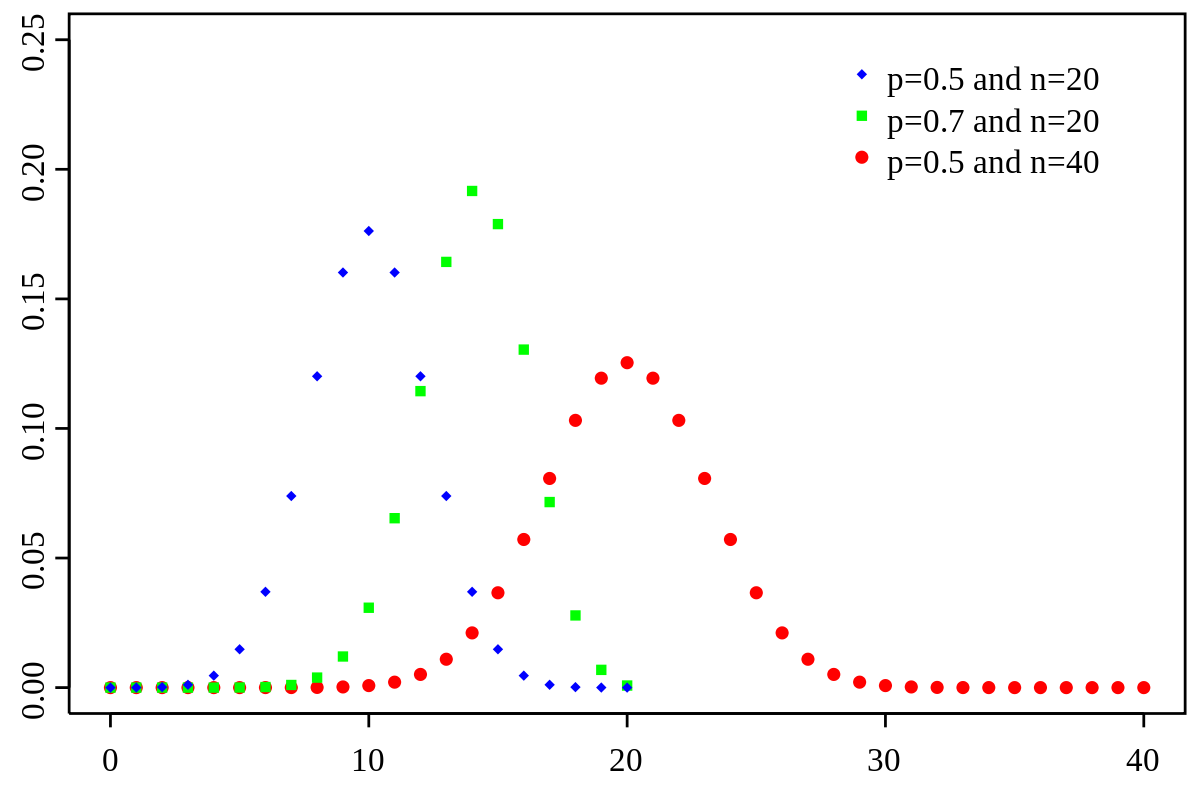
\includegraphics[scale=0.3]{imagen1.png}
    \caption{Imagen 1 distribución Binomial}
    \end{figure}

\newpage

\section{diagramas conmutativos}
\[
\xymatrix{
A & B \ar[rd] & C & D & E\\
\alpha & \gamma & \beta & \delta
& \epsilon
}
\]
\[
\xymatrix{
A & B \ar@{.>}[ld] \ar@{--}@(dr,ul)[r]
& C & D \ar@{->>}[d] & E \ar@{<-}[d]
& F \\ \alpha & \beta \ar@/^/[r] \ar@/_/[r]
& \gamma & \delta & \epsilon & \phi
}
\]
\newpage
\section{cajas}
\colorbox{yellow}{Este texto está en una caja de color amarillo} \\
\colorbox{green}{$\sqrt{\frac{x^2}{2}}$} \\ 
\fcolorbox{marron}{violeta}{\textcolor{gris-oscuro}{La fórmula para ds}}\\
\fcolorbox{red}{yellow}{\textcolor{cafe}{hola}} \\ 

\newpage

\section{MATEMÁTICAS ACTUARIALES}
\subsection{tabla de mortalidad}
\begin{tabular}{|l|}
\hline
$l_{x}$: Número de vivos de edad exacta $x$\\
$d_{x}$: Número de muertes ocurridas entre
las edades $x$ y $x+1$\\
${}_nd_{x}$: Número de muertes ocurridas entre
las edades $x$ y $x+n$\\
$p_{x}$: Probabilidad de que una persona de edad
exacta $x$ sobreviva 1 año más\\
${}_np_{x}$: Probabilidad de que una persona de
edad $x$ sobreviva $n$ años más\\
$q_{x}$: Probabilidad de que una persona de edad
$x$ muera entre las edades $x$ y $x+1$\\
${}_nL_{x}$ Años  persona  vividos entre las edades

$x$ y $x+n$\\

$T_x$: Años persona vividos entre las edades $x$
y $w$\\
$\mathring{e}_x$: Esperanza de vida a la edad $x$\\ \hline
\end{tabular}
\subsection{Anualidades contingentes}
\begin{tabular}{|l|}
\hline
Dotal puro $n$ años ${}_nE_x$\\
Anualidad vitalicia vencida $a_x$\\
Anualidad vitalicia anticipada
$\ddot{a}_x$\\
Anualidad vencida temporal $n$
años 
$a_{x:n}$\\
Anualidad anticipada temporal $n$
años $\ddot{a}_{x:n}$ \\ \hline
\end{tabular}
\newpage 
\section{Ejercicio 39  de la sección 1.6 Blanchard}
Suponga que desea modelar una población con 
        una ecuación diferencial de la forma $\frac{dP}{dt}=f(P)$,
        donde $P(t)$ es la población en el tiempo $t$.\\ 
        Los experimentos han sido realizadas sobre la población 
        que dan la siguiente información:
        \begin{itemize}
            \item Los únicos puntos de equilibrio son P = 0,
            P = 10 y P = 50. 
            \item Si la población es 100, la población disminuye. 
            \item Si la población es de 25, la población aumenta. 
        \end{itemize}
        \begin{itemize}
            \item[(a)] Dibuje las líneas de fase posibles para este sistema
            para $P>0$ (hay dos)
            \item[(b)] Dé un bosquejo aproximado de las funciones correspondientes
            $f(p)$ para cada uno de sus lineas de fase.
            \item[(c)] Dé una fórmula para las funciones $f(p)$ cuya gráfica 
            concuerde(cualitativamente) con los bosquejos aproximados
            de la parte (b) para cada una de sus líneas de fase.  
        \end{itemize} 
        \textbf{Desarrollo}\\ 
        \textbf{a)}\\ 
        \begin{center}
            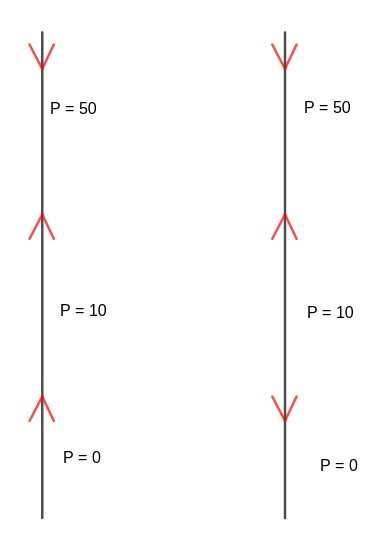
\includegraphics[scale=0.3]{lineas de fase.jpeg}
        \end{center}
        \textbf{b) y c)} \\ Primera linea de fase
        \begin{center}
            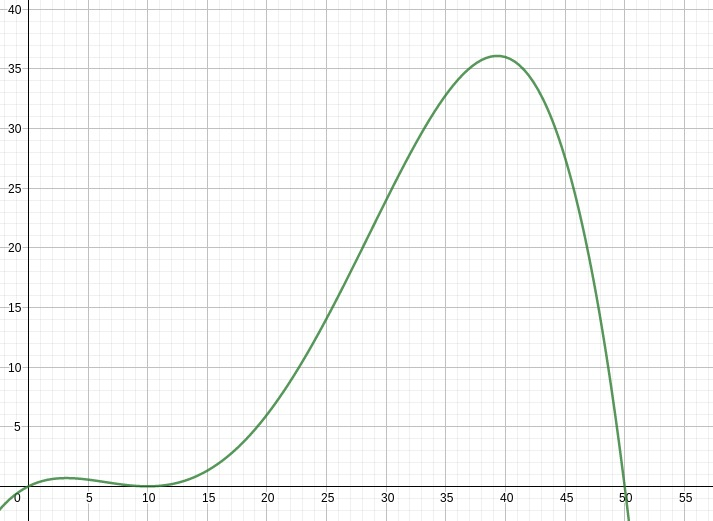
\includegraphics[scale=0.3]{1g.jpeg}
        \end{center}
        $f(P)=\frac{1}{10000}P(P-10)^{2}(50-P)$ 
\section{Ejercicio 25 de la sección 1.9 Blanchard}
Un tanque de 400 galones inicialmente 
contiene 200 galones de agua que contienen 2 
partes por mil millones en peso de dioxina, 
un carcinógeno extremadamente potente. 
Supongamos que el agua contiene
5 partes por mil millones de dioxina fluyen 
hacia la parte superior del tanque a una 
velocidad de 4 galones por minuto. 
El agua del tanque se mantiene bien 
mezclada y se extraen 2 galones por minuto del 
fondo del tanque. ¿Cuánta dioxina hay en el 
tanque cuando está lleno? \\ 
$Q(t)$ cantidad de dioxiona en un tiempo t. 
$c_{e} = 5 \frac{partes}{mil millones}$  \\ 
$v_{e} = 4 \frac{galones}{minuto}$ \\ 
$v_{s}=2 \frac{galones}{minuto}$ \\ 
$v = v_{o}+(v_{e}-v_{s})t=200+(4-2)t = 200 +2t$ \\ 
$c_{s}=\frac{Q_{(t)}}{v} = \frac{Q_{(t)}}{200+2t}$
\\ 
entonces, $Q'_{t}+\frac{2}{200+2t}Q=20$\\
$Q'_{t}+\frac{1}{100+t}Q=20$
\\
Como, $Q(t) =\underbrace{Q_{1}(t)}_{homogenea} +\underbrace{Q_{2}(t)}_{particular}$ 
\subsection{Homogenea}
\begin{equation*}
    \begin{split}
        Q'(t) + \frac{1}{100+t} = 0\\
        Q_{1} (t)=e^{-\int_{t_{0}}^{t}(\frac{1}{100+T}dT)Q_{0}} \\
        = e^{(\ln{(100+t_{0})}-\ln{(100+t)})} \\
        = e^{\ln{(\frac{100+t_{0}}{100+t})}Q_{0}} \\
        = \frac{100+t_{0}}{100+t}Q_{0}
    \end{split}
    \end{equation*}
\subsection{Particular}
\begin{equation*}
    \begin{split}
        Q'(t)+\frac{1}{100+t}Q=20 \\
        Q_{2}(t)= \frac{100+t_{0}}{100+t}\int_{t_{0}}^{t}\frac{100+T}{100+t_{0}}20dT \\ 
        = \frac{20}{100+t}\int_{t_{0}}^{t}100+TdT \\ 
        = \frac{20}{100+t}(100t-100t_{0}+\frac{t^{2}-t_{0}^{2}}{2})
    \end{split}
\end{equation*}
Ahora, cuando $t_{0}=0$ y $Q_{0}=2$
obtendremios una solución especifica
\begin{equation*}
    \begin{split}
        Q(t) = \frac{100}{100+t}(2) + \frac{20}{100+t}(100t+\frac{t^{2}}{2})\\
        = \frac{200+2000t+10t^{2}}{100+t}
    \end{split}
\end{equation*}
Entonces \\
\begin{equation*}
    \begin{split}
        v (t) = 200 + 2t \\
        400 = 200 + 2t \\
        200 = 2t \\
        100 = t
    \end{split}
\end{equation*}
\begin{equation*}
    \begin{split}
        Q_{(100)}=\frac{200+2000(100)+10(100)^{2}}{100+100} \\
        =1501
    \end{split}
\end{equation*}
\section{Ejercicio sobre la ecuación de Bessel}
Sean $x_{1}=x_{1}(t)$ y $x_{2}=x_{2}(t)$ 
las soluciones de la ecuación de Bessel
\begin{center}
    $2t^{2}x^{''}+tx^{'}+(t^{2}-n^{2})x=0$, $n>0$ constante,
\end{center}
definidas sobre el intervalo $0<t<\infty$, y que satisfacen las condiciones 
$x_{1}(1)=1 $, $x_{1}^{'}(1)=0$ , $x_{2}(1)=0$, $x_{2}^{'}=1$, Demuestre 
que $x_{1}(t)$ y $x_{2}(t)$ forman un conjunto fundamental de soluciones en 
$(o, \infty)$.
\begin{thm}
\textbf{Criterio para conjunto fundamental de soluciones} 
Sean $x_{1}=x_{1}(t)$ y $x_{2}=x_{2}(t)$ dos soluciones de la ecuacion diferencial, $t\in J$ entonces los tres condiciones siguientes son equivalentes. 
\begin{enumerate}
    \item $x_{1}(t)$ y $x_{2}(t)$ forman un conjunto fundamental de soluciones 
    \item $w_{t}=w(x_{1},x_{2}) \not = 0$ para todo $t \in J$
    \item $w(t_{0}) \not = 0 $ para algún $t_{0}$ en $J$
\end{enumerate} 
\textbf{$3 \to 1$} \\
Suponga que para dos, constantes $c_{1}$ y $c_{2}$ se tiene:
\begin{equation*}
    x(t) = c_{1}x_{1}(t) + c_{2}x_{2}(t) = 0, \forall t \in J
\end{equation*}
entonces, 
\begin{equation*}
    x'(t) = c_{1}x'_{t} + c_{2}x'_{2}(t) = 0, \forall t \in J
\end{equation*}
En particular para $t = t_{0}$, 
\begin{equation*}
    c_{1}x_{1}(t_{0}) + c_{2}x_{2}(t_{0}) = 0
\end{equation*}
\begin{equation*}
    c_{1}x'(t_{0}) + c_{2}x'_{2}(t_{0}) = 0 
\end{equation*}
como $w_(t_{0}) \not = 0$ es el determinate de la matriz de coeficientes de anterior 
sistema de ecuaciones se concluye que $c_{1} = c_{2} = 0$ , lo que prueba la independencia 
lineal de $x_{1}$ y $x_{2}$.$\spadesuit$
\end{thm}
\subsection*{Solución del ejercicio}
Para dar solucionar el ejercicico, vamos a usar del teorema anterior el númeral (3), y entonces probaremis que $x_{1}(t)$ y $x_{2}(t)$ forman un conjunto fundamental de soluciones
\begin{itemize}
    \item[*] La ecucación de Bessel es homogenea 
    \item[*] Conjunto solución $(0, \infty)$
    \item[*] $t_{0}=1$ y $1 \in (0, \infty)$
    \item[*] $w(1) = w(x_{1}(1),x_{2}(1))= det
        \begin{pmatrix}
            x_{1}(1) & x_{2}(1)  \\
            x'_{1}(1) & x'_{2}(1)  \\
        \end{pmatrix} =  x_{1}(1) x'_{2}(1) -  x'_{1}(1) x_{2}(1) = (1 \cdot 1) -(0 \cdot 0) = 1 \not = 0$
\end{itemize}
$\to x_{1}(t)$ y $ x_{2}(t)$ forman un conjunto fundamental de soluciones en $(0, \infty)$.
$\spadesuit$ 
\section{Grupos simples finito y campos finitos}
Los conceptos sobre grupos simples, los campos finitos y las geometrías finitas 
tardaron más de 100 años en desarrollarse.\newline

Se centran en el concepto de grupo lineal que llego a su madurez en el libro
``\textit{Linear Group, with an Exposition of the Galois Field Theory of Dickson}" (1910).
\newline

Actualmente se define un grupo lineal como un grupo de matrices con entradas en un 
campo. Las matrices fueron introducidas por Cayley (1855).
El concepto de campo finito se remonta a Galois. Tomemos el campo 
$\mathbb{F}_p = \{0, 1, 2, ..., p-1 \}$, existe el campo $\mathbb{F}_{p^n}$, 
para cada número natural $n$, cuyos elementos polinomios de grado $n-1$ con 
 en $\mathbb{F}_p$.
\\ 
\textbf{Ejemplo} \\
\begin{tabular}{|l|}
    \hline 
    Consideremos $\mathbb{F}_4 = \mathbb{F}_{2^2} = \{0, 1, x, x+1 \}$\\
    bajo la adición y multiplicación mod $2$. Note que, el campo \\
    $\mathbb{F}_4 = \mathbb{F}_{2^2}$ se construye:\\
    $\mathbb{F}_4 = \mathbb{F}_2\left[x \right] / \left<x^2 + x + 1 \right>$ \\ \hline
\end{tabular} \\
Se deduce que hay campos con $4$, $8$ y $9$ elementos porque $4=2^2$, $8=2^3$ y $9=3^2$.

Las transformaciones de las lineas proyectivas sobre campos nos dan un nuevo grupo simple

\begin{itemize}
    \item<1-> $PSL(2, 4) = PGL(2, 4)$ tiene $5\cdot 4\cdot 3 = 60$ elementos, y resulta que es isomorfo a $A_5$.\newline
    
    \item<2-> $PSL(2, 9)$ tiene $10 \cdot 9 \cdot 8/2 = 360$ elementos, y resulta ser isomorfo a $A_6$.\newline
    
    \item<3-> $PSL(2, 8) = PGL(2, 8)$ tiene $9 \cdot 8 \cdot 7 = 504$ elementos, y es un nuevo grupo simple, descubierto por Cole (1893).
    
\end{itemize} 
Moore demostro:

\begin{itemize}
    \item Todo campo finito es isomorfo a uno de los campos de Galois $\mathbb{F}_{p^n}$.\newline
    
    \item Todos los grupos $PSL(2,np)$ son simples cuando $p>3$ y $n>1$.\newline
\end{itemize}
Rescribiendola,
\\
\begin{tabular}{|l|}
    \hline
    ``Todos los grupos $PSL(2,p^n)$ son simples cuando $p^n>3$." \\ \hline
\end{tabular}
\\
De forma general,
\\
\begin{tabular}{|l|}
    \hline
    ``$PSL(m,q)$ es simple para todo $m,q\geq 2$ excepto $(m,q) = (2,2), (2,3)$." \\ \hline
\end{tabular}
\\ 
En conclusión, 
\begin{Def}
    $PSL(m,q)$ es el grupo de matrices $m\times m$ con entradas en $\mathbb{F}_q$ y 
    determinante $1$ cocientado por el subgrupo formado por la matriz identidad y su negativo.
\end{Def}
La geometría se puso al día en 1905 cuando Veblen definió el espacio proyectivo $m-$dimensional sobre el campo $\mathbb{F}_q$.\newline

Se descubrió que grupos como el ``grupo de rotación de $\mathbb{R}^n$" tienen homólogos finitos que suelen ser grupos simples.\newline

En 1860, surgieron cinco grupos simples finitos de la nada. Estos grupos se conocen como los grupos de Mathieu, en honor a su descubridor ``Emile Mathieu".
\section{Los grupos de Mathieu}
Un grupo se llama grupo $k-$transitivo, si existe un conjunto de elementos sobre los que el grupo actúa fiel (monomorfismo) y $k-$transitivamente.\newline

Si los elementos de G permutan un cierto conjunto S, entonces\newline
\begin{itemize}
    \item $G$ se llama $1-$transitivo si cualquier miembro de $S$ puede ser enviado a cualquier otro miembro de $S$ mediante una permutación en $G$.\newline
    
    \item  $G$ se llama $2-$transitivo si cualquier par ordenado de miembros de $S$ puede ser a cualquier otro par ordenado de miembros de $S$ por un miembro de $G$.
\end{itemize}
\begin{Def}
    El grupo $G$ actúa sobre el conjunto $S$ si
\begin{equation*}
\begin{split}
    \psi:G\times S &\longrightarrow S\\
       (g,x) &\longmapsto g\cdot x
\end{split}
\end{equation*}
\begin{itemize}
    \item[1.] $\psi(e,x) = e\cdot x = x$ para todo $x\in S$.
    \item[2.] $\psi(g_2,\psi(g_1,x)) = \psi(g_2,g_1\cdot x) = (g_2g_1)\cdot x = \psi(g_2g_1, x) $
\end{itemize}
\end{Def}
\begin{Ej}
    El grupo alterno $A_n$ es $k-$transitivo para números impares $k\leq n$.
\end{Ej}
\begin{itemize}
    \item<1-> Mathieu descubrió (1861, 1873) cuatro grupos de permutación que son 4 o 5-transitivos, y un grupo relacionado que es 3-transitivo.\newline
    
    \item<2-> Los cincos grupos de Mathieu se denominan $M_{11}$, $M_{12}$, $M_{22}$, $M_{23}$ y $M_{24}$.\newline

    \begin{tabular}{|c|c|l|}
       \hline
       Grupo & Transitividad & Orden    \\ \hline
       $M_{11}$ & 4 & 11$\cdot$10$\cdot$9$\cdot$8   \\ 
       $M_{12}$ & 5 & 12$\cdot$11$\cdot$10$\cdot$9$\cdot$8     \\ 
       $M_{22}$ & 3 & 22$\cdot$21$\cdot$20$\cdot$16$\cdot$3     \\ 
       $M_{23}$ & 4 & 23$\cdot$22$\cdot$21$\cdot$20$\cdot$16$\cdot$3     \\ 
       $M_{24}$ & 5 & 24$\cdot$23$\cdot$22$\cdot$21$\cdot$20$\cdot$16$\cdot$3     \\   \hline
    \end{tabular}

\end{itemize}
?`Cuál es la mejor manera de codificar los mensajes para que los errores puedan ser detectados y corregidos?\newline

Un mensaje se divide en ``caracteres", que son secuencias de 0s y 1s (secuencias binarias) de una determinada longitud fija k.\newline

El objetivo de la teoría de la codificación es conseguir la máxima corrección de errores con el mínimo aumento de la longitud del mensaje.\newline
\begin{Ej}
    Para $d = 3$ y $k = 7$ es la longitud mínima que se puede utilizar para obtener 16 caracteres, y esto se consigue con el siguiente código: 
\begin{equation*}
\begin{matrix}
0000000 & 0100101 & 1000110 & 1100011 \\
0001111 & 0101010 & 1001001 & 1101100 \\
0010011 & 0110110 & 1010101 & 1110000 \\
0011101 & 0111001 & 1011010 & 1111111 \\
\end{matrix} 
\end{equation*}
\end{Ej}
Este código se debe a Hamming (1950), y se conoce como \textit{código Hamming} $(7, 4)$. Un código más notable es el código $(23, 12)$ de Golay (1949). El \textit{código de Golay} consiste en $2^{12} = 4096$ secuencias binarias de longitud $23$, dos de las cuales difieren en al menos siete dígitos (tres dígitos erróneos). 
\begin{itemize}
    \item<1-> Las simetrías del código pueden realizarse mediante un grupo de transformaciones lineales del espacio $\mathbb{F}_{2^{32}}$, y este grupo de simetría resulta ser nada menos que $M_{23}$.\newline
    
    \item<2-> El grupo $M_{24}$ aparece cerca, como el grupo de simetría de un subconjunto relacionado de $\mathbb{F}_{2^{24}}$, el llamado \textit{código de Golay extendido}.\newline
    
    \item<3-> Estos descubrimientos se deben a Paige (1957) y Assmus y Mattson (1966). 
\end{itemize}
\section{Grupos continuos}
La teoría de los grupos continuos fue creada por el matemático noruego Sophus Lie en la 
década de 1870. Inicialmente, su objetivo era desarrollar una teoría de ecuaciones
diferenciales como la teoría de ecuaciones polinómicas de Galois. Vio que cada 
ecuación diferencial tiene un grupo, análogo al grupo de Galois pero “continuo”
en lugar de finito, y que los grupos “simples” presentan un obstáculo para la 
solución. 
\\ 
El ejemplo más fácil de entender de un grupo continuo es la recta numérica R, bajo 
la operación de suma. Este grupo es “continuo” en el sentido de que la operación de grupo $x , t \to x+y$, y también la operación inversal de grupo $x \to -x$, es una 

función continua. Un ejemplo relacionado es el círculo unitario
\begin{equation*}
    \mathbb{S}^{1}=\{z : |z|=1\}
\end{equation*}
Podemos interpretar un 
miembro z de SO(2) como una rotación del plano, porque
\begin{equation*}
    z = \cos{\theta}+ i \sin{\theta}\text{, para algun } \theta
\end{equation*} 
El primer grupo continuo realmente interesante es $SO(3)$, el
grupo de rotación del espacio tridimensional $\mathbb{R}^{3}$. Si tomamos
una rotación $r$ de $\mathbb{R}^{3}$ dada por un eje $A$ que pasa por $O$ y un
giro de ángulo $\theta$ alrededor de $A$, entonces ni siquiera es obvio
que las rotaciones espaciales formen un grupo. Dada una
rotación $r$ con eje $A$ y ángulo $\theta$, y una rotación $s$ con eje $B$ 
ángulo $\varpi$, ¿podemos estar seguros de que la combinación $sr$ tiene
incluso un eje $C$ y un ángulo $X$ bien definidos? La respuesta es
(sí) aparentemente fue encontrada por primera vez por Euler
(1776), pero ahora podemos encontrar esta respuesta mucho más
fácilmente. El truco consiste en ver cada rotación como un
producto de dos reflexiones, como se muestra en la siguiente figura. 
\newpage
\begin{figure}[h]
    \centering
    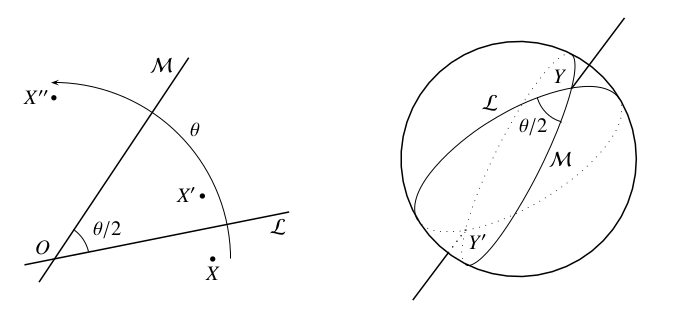
\includegraphics[scale=0.5]{23.3-1.png}
    \caption{Rotación a través de un par de reflexiones}
    \end{figure}
    Supongamos ahora que queremos encontrar el resultado de
    realizar la rotación $r$ de la esfera, con eje que pasa por $P$ y
    ángulo $\theta$, luego la rotación $s$ con eje
    a través de $Q$ y el ángulo $\varphi$. Haciendo uso de nuestra
    libertad para elegir los grandes círculos de reflexión,
    realizamos $r$ por el par de reflexiones en los grandes
    círculos $L$ y $M$ a través de $P$ que están separados por un ángulo $\theta/2$, donde $M$ pasa a través de $P$ y $Q$. 
    \begin{figure}[h]
        \centering
        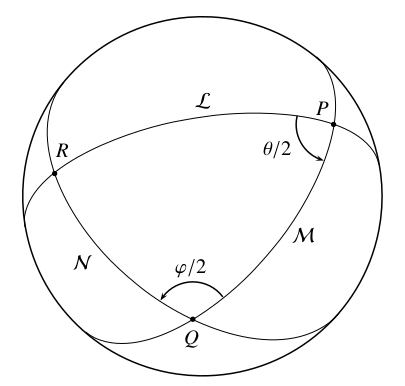
\includegraphics[scale=0.5]{23.3-2.png}
        \caption{Hallar el producto de rotaciones}
        \end{figure}
\newpage
\begin{thebibliography}{X}
    \bibitem{AATA} \textsc{Thomas W. Judson }  \textit{Algebra Abstracta : Teoría y Aplicaciones} \\
    \url{http://abstract.ups.edu/aata-es/section-sylow-theorems.html}
    \bibitem{TDP} \textsc{Tablas de probabilidad} \\ 
    \url{https://www.uv.es/montes/nau_gran/tablas.pdf} \\ 
    \url{https://www.superprof.es/apuntes/escolar/matematicas/probabilidades/distribucion-normal/tabla-de-la-distribucion-normal.html}
    \bibitem{OPM} \textsc{Operaciopnes con matrices} \\ 
    \url{https://www.superprof.es/apuntes/escolar/matematicas/algebralineal/matrices/operaciones-con-matrices.html}
    \bibitem{DC} \textsc{Misraim Guitiérrez} \textit{Introducción al \LaTeX} \\ 
    \url{https://sistemas.fciencias.unam.mx/~misraim/notas.pdf}
    \bibitem{LA} \textsc{Dept. d'informática, universitat de valéncia } \textit{\LaTeX avanzado pauqetes y herramientas para gráficos} 
    \bibitem{}
\end{thebibliography}

\end{document}